%
%===============>>  ГРУППА 9-1 МОДУЛЬ 8  <<=============
%
\setmodule{8}

%BEGIN_FOLD % ====>>_____ Занятие 1 _____<<====
\begin{class}[number=1]
	\begin{listofex}
		\item Какие из следующих утверждений верны?
		\begin{tasks}(1)
			\task Через точку, не лежащую на данной прямой, можно провести прямую, параллельную этой
			прямой.
			\task Треугольник со сторонами \( 1 \), \( 2 \), \( 4 \) существует.
			\task В любом параллелограмме есть два равных угла.
		\end{tasks}
		\item Какие из следующих утверждений верны?
		\begin{tasks}(1)
			\task Любые два прямоугольных треугольника подобны.
			\task Если катет и гипотенуза прямоугольного треугольника равны соответственно \( 6 \) и \( 10 \), то второй катет этого треугольника равен \( 8 \).
			\task Стороны треугольника пропорциональны косинусам противолежащих углов.
			\task Квадрат любой стороны треугольника равен сумме квадратов двух других сторон без удвоенного произведения этих сторон на косинус угла между ними.
		\end{tasks}	
	\item Укажите номера верных утверждений.
	\begin{tasks}(1)
		\task Если угол равен \( 45\degree \), то вертикальный с ним угол равен \( 45\degree \).
		\task Любые две прямые имеют ровно одну общую точку.
		\task Через любые три точки проходит ровно одна прямая.
		\task Если расстояние от точки до прямой меньше \( 1 \), то и длина любой наклонной, проведенной из данной точки к прямой, меньше \( 1 \).
	\end{tasks}
	\item Укажите номера верных утверждений.
	\begin{tasks}(1)
		\task Если при пересечении двух прямых третьей прямой соответственные углы равны \( 65\degree \), то эти две прямые параллельны.
		\task Любые две прямые имеют не менее одной общей точки.
		\task Через любую точку проходит более одной прямой.
		\task Любые три прямые имеют не менее одной общей точки.
	\end{tasks}
	\item Укажите номера верных утверждений.
	\begin{tasks}(1)
		\task  Если при пересечении двух прямых третьей прямой внутренние накрест лежащие углы составляют в сумме \( 90\degree \), то эти две прямые параллельны.
		\task Если угол равен \( 60\degree \), то смежный с ним равен \( 120\degree \).
		\task Если при пересечении двух прямых третьей прямой внутренние односторонние углы равны \( 70\degree \) и \( 110\degree \), то эти две прямые параллельны.
		\task Через любые три точки проходит не более одной прямой.
	\end{tasks}
	\item Укажите номера верных утверждений.
	\begin{tasks}(1)
		\task Вписанные углы, опирающиеся на одну и ту же хорду окружности, равны.
		\task Если радиусы двух окружностей равны \( 5 \) и \( 7 \), а расстояние между их центрами равно \( 3 \), то эти окружности не имеют общих точек.
		\task Если радиус окружности равен \( 3 \), а расстояние от центра окружности до прямой равно \( 2 \), то эти прямая и окружность пересекаются.
		\task Если вписанный угол равен \( 30\degree \), то дуга окружности, на которую опирается этот угол, равна \( 60\degree \).
	\end{tasks}
	\item Укажите номера верных утверждений.
	\begin{tasks}(1)
		\task Через любые три точки проходит не более одной окружности.
		\task Если расстояние между центрами двух окружностей больше суммы их диаметров, то эти окружности не имеют общих точек.
		\task Если радиусы двух окружностей равны \( 3 \) и \( 5 \), а расстояние между их центрами равно \( 1 \), то эти окружности пересекаются.
		\task Если дуга окружности составляет \( 80\degree \), то вписанный угол, опирающийся на эту дугу окружности, равен \( 40\degree \).
	\end{tasks}
	\item Решите системы уравнений:
	\begin{tasks}(2)
		\task \( \begin{cases}
			(2x+3)^2=5y,\\
			(3x+2)^2=5y
		\end{cases} \)
		\task \( \begin{cases}
			x-y=-5,\\
			x^2-2xy-y^2=17
		\end{cases} \)
		\task \( \begin{cases}
			x^2+3x+y^2=2,\\
			x^2+3x-y^2=-6
		\end{cases} \)
		\task \( \begin{cases}
			3x-y=2,\\
			x^2-4x+8=y
		\end{cases} \)
		\task \( \begin{cases}
			3x+y=5,\\
			\dfrac{x+2}{y}+\dfrac{y}{2}=-1
		\end{cases} \)
	\end{tasks}
	\item Решите уравнение \( (x^2-9)^2+(x^2-2x-15)^2=0 \)
	\end{listofex}
\end{class}
%END_FOLD

%BEGIN_FOLD % ====>>_____ Занятие 2 _____<<====
\begin{class}[number=2]
	\begin{listofex}
			\item Укажите номера верных утверждений.
		\begin{tasks}(1)
			\task Около всякого треугольника можно описать не более одной окружности.
			\task В любой треугольник можно вписать не менее одной окружности.
			\task Центром окружности, описанной около треугольника, является точка пересечения биссектрис.
			\task Центром окружности, вписанной в треугольник, является точка пересечения серединных перпендикуляров к его сторонам.
		\end{tasks}
		\item Укажите номера верных утверждений.
		\begin{tasks}(1)
			\task Около любого правильного многоугольника можно описать не более одной окружности.
			\task Центр окружности, описанной около треугольника со сторонами, равными \( 3 \), \( 4 \), \( 5 \), находится на стороне этого треугольника.
			\task Центром окружности, описанной около квадрата, является точка пересечения его диагоналей.
			\task Около любого ромба можно описать окружность.
		\end{tasks}
		\item Укажите номера верных утверждений.
		\begin{tasks}(1)
			\task Окружность имеет бесконечно много центров симметрии.
			\task Прямая не имеет осей симметрии.
			\task Правильный пятиугольник имеет пять осей симметрии.
			\task Квадрат не имеет центра симметрии.
		\end{tasks}
		\item Укажите номера верных утверждений.
		\begin{tasks}(1)
			\task Правильный шестиугольник имеет шесть осей симметрии.
			\task Прямая не имеет осей симметрии.
			\task Центром симметрии ромба является точка пересечения его диагоналей.
			\task Равнобедренный треугольник имеет три оси симметрии.
		\end{tasks}
	\newpage
		\item Укажите номера верных утверждений.
		\begin{tasks}(1)
			\task Центром симметрии прямоугольника является точка пересечения диагоналей.
			\task Центром симметрии ромба является точка пересечения его диагоналей.
			\task Правильный пятиугольник имеет пять осей симметрии.
			\task Центром симметрии равнобедренной трапеции является точка пересечения ее диагоналей.
		\end{tasks}
		\item Укажите номера верных утверждений.
		\begin{tasks}(1)
			\task Если катет и гипотенуза прямоугольного треугольника равны соответственно \( 6 \) и \( 10 \), то второй катет этого треугольника равен \( 8 \).
			\task Любые два равнобедренных треугольника подобны.
			\task Любые два прямоугольных треугольника подобны.
			\task Треугольник \( ABC \), у которого \( AB=3 \), \( BC=4 \), \( AC=5 \), является тупоугольным.
		\end{tasks}
		\item Решите системы неравенств:
		\begin{tasks}(2)
			\task \( \begin{cases}
				 7(3x+2)-3(7x+2)>2x ,\\
				(x-5)(x+8)<0
			\end{cases} \)
			\task \( \begin{cases}
				4(9x+3)-9(4x+3)>3x,\\
				(x-2)(x+9)<0
			\end{cases} \)
			\task \( \begin{cases}
			(6x+2)-6(x+2)>2x,\\
			(x-7)(x+6)<0
			\end{cases} \)
			\task \( \begin{cases}
			5(2x+3)-2(5x+3)>3x,\\
			(x-6)(x+2)<0
			\end{cases} \)
			\task \( \begin{cases}
			\dfrac{10-2x}{3+(5-2x)^2}\ge0,\\
			2-7x\le14-3x
			\end{cases} \)
			\task \( \begin{cases}
			\dfrac{3-x}{1+(5-x)^2}\ge0,\\
			8-7x\le24-3x
			\end{cases} \)
		\end{tasks}
		\item Решите уравнение \( (x^2-9)^2+(x^2-2x-15)^2=0 \)
	\end{listofex}
\end{class}
%END_FOLD

%BEGIN_FOLD % ====>>_ Домашняя работа 1 _<<====
\begin{homework}[number=1]
	\begin{listofex}
		\item Какие из следующих утверждений верны?
		\begin{tasks}(1)
			\task Около всякого треугольника можно описать не более одной окружности.
			\task В любой треугольник можно вписать не менее одной окружности.
			\task Центром окружности, описанной около треугольника, является точка пересечения биссектрис.
			\task Центром окружности, вписанной в треугольник, является точка пересечения серединных перпендикуляров к его сторонам.
		\end{tasks}
		\item Какие из следующих утверждений верны?
		\begin{tasks}(1)
			\task Косинус острого угла прямоугольного треугольника равен отношению гипотенузы к прилежащему к этому углу катету.
			\task Диагонали ромба перпендикулярны.
			\task Существуют три прямые, которые проходят через одну точку.
		\end{tasks}
		\item Какие из следующих утверждений верны?
		\begin{tasks}(1)
			\task Все хорды одной окружности равны между собой.
			\task Треугольника со сторонами \( 1 \), \( 2 \), \( 4 \) не существует.
			\task Все углы прямоугольника равны.
		\end{tasks}
		\item Решите системы уравнений:
		\begin{tasks}(2)
			\task \( \begin{cases}
				5x+y=-13,\\
				x^2+y^2=13
			\end{cases} \)
			\task \( \begin{cases}
				2x^2+y^2=36,\\
				8x^2+4y^2=36x
			\end{cases} \)
		\end{tasks}
		\item Решите системы неравенств:
		\begin{tasks}(2)
			\task \( \begin{cases}
				\dfrac{6-3x}{4+(9-2x)^2}\ge0,\\
			 	5-8x\le23-5x
			\end{cases} \)
			\task \( \begin{cases}
				8(3x+5)-3(8x+5)>5,\\
				(x-8)(x+1)<0
			\end{cases} \)
		\end{tasks}
		\item Имеются два сосуда, содержащие \( 30 \) кг и \( 20 \) кг раствора кислоты различной концентрации. Если их слить вместе, то получим раствор, содержащий \( 81\% \) кислоты. Если же слить равные массы этих растворов, то полученный раствор будет содержать \( 83\% \) кислоты. Сколько килограммов кислоты содержится во втором растворе?
	\end{listofex}
\end{homework}
%END_FOLD

%BEGIN_FOLD % ====>>_____ Занятие 3 _____<<====
\begin{class}[number=3]
	\begin{listofex}
		\item Один из корней уравнения \( 3x^2+5x-2m=0 \) равен \( -1 \). Найдите второй корень.
		\item Решите уравнения:
		\begin{tasks}(2)
			\task \( \dfrac{2x^2+7x+3}{x^2-9}=1 \)
			\task \( x^6=(6x-5)^3 \)
			\task \( (x+2)^4-4(x+2)^2-5=0 \)
			\task \( \dfrac{1}{(x-2)^2}-\dfrac{1}{x-2}-6=0 \)
		\end{tasks}
		\item Один мастер может выполнить заказ за \( 12 \) часов, а другой --- за \( 6 \) часов. За сколько часов выполнят заказ оба мастера, работая вместе?
		\item На изготовление \( 99 \) деталей первый рабочий тратит на \( 2 \) часа меньше, чем второй рабочий на изготовление \( 110 \) таких же деталей. Известно, что первый рабочий за час делает на \( 1 \) деталь больше, чем второй. Сколько деталей в час делает второй рабочий?
		\item На изготовление \( 231 \) детали ученик тратит на \( 11 \) часов больше, чем мастер на изготовление \( 462 \) таких же деталей. Известно, что ученик за час делает на \( 4 \) детали меньше, чем мастер. Сколько деталей в час делает ученик?
		\item Первая труба пропускает на \( 1 \) литр воды в минуту меньше, чем вторая. Сколько литров воды в минуту пропускает первая труба, если резервуар объемом \( 110 \) литров она заполняет на \( 1 \) минуту дольше, чем вторая труба?
		\item Первая труба пропускает на \( 5 \) литров воды в минуту меньше, чем вторая. Сколько литров воды в минуту пропускает вторая труба, если резервуар объемом \( 375 \) литров она заполняет на \( 10 \) минут быстрее, чем первая труба заполняет резервуар объемом \( 500 \) литров?
	\end{listofex}
\end{class}
%END_FOLD

%BEGIN_FOLD % ====>>_____ Занятие 4 _____<<====
\begin{class}[number=4]
	\begin{listofex}
		\item Постройте график:
		\[ y=	 \left\{
		\begin{array}{l}
			1,5x-3, \quad x<2,\\
			-1,5x+3, \quad 2\leq x\leq3,\\
			3x-10,5, \quad x>3.
		\end{array}
		\right. \]
		и определите, при каких значениях \( m \) прямая \( y=m \) имеет с графиком ровно две общие точки.
		\item  Постройте график функции
		\[y=	 \left\{
		\begin{array}{l}
			2x+1, \quad x<0,\\
			-1,5x+1, \quad 0\leq x<2,\\
			x-4, \quad x\geq 2
		\end{array}
		\right. \]
		и определите, при каких значениях \( m \) прямая \( y=m \) имеет с графиком ровно две общие точки.
		\item Постройте график функции
		\[y=	 \left\{
		\begin{array}{l}
			x^2+2x+3, \quad x\leq-3,\\
			x+9, \quad x>-3
		\end{array}
		\right. \]
		и определите, при каких значениях \( m \) прямая \( y=m \) имеет с графиком ровно две общие точки.
		\item Построить график функции \( y=x-|2x+1|-2 \). Найти точки пересечения данного графика с графиком функции \( y=x-5 \).
		\item Постройте график функции \( y=x^2-3|x|-x \)  и определите, при каких значениях \( c \)  прямая \( y=c \)  имеет с графиком три общие точки.
	\end{listofex}
\end{class}
%END_FOLD

%BEGIN_FOLD % ====>>_ Домашняя работа 2 _<<====
\begin{homework}[number=2]
	\begin{listofex}
		\item Решите уравнение: \[\dfrac{1}{x^2}+\dfrac{4}{x}-12=0\]
		\item Две трубы наполняют бассейн за \( 8 \) часов \( 45 \) минут, а одна первая труба наполняет бассейн за \( 21 \) час. За сколько часов наполняет бассейн одна вторая труба?
		\item Первая труба пропускает на \( 5 \) литров воды в минуту меньше, чем вторая труба. Сколько литров воды в минуту пропускает вторая труба, если резервуар объёмом \( 180 \) литров она заполняет на \( 3 \) минуты быстрее, чем первая труба?
		\item Постройте график функции \( y=|x|(x+1)-6x \) и определите, при каких значениях \( m \) прямая \( y=m \) имеет с графиком ровно две общие точки.
	\end{listofex}
\end{homework}
%END_FOLD

%BEGIN_FOLD % ====>>_____ Занятие 5 _____<<====
\begin{class}[number=5]
	\begin{listofex}
		\item Постройте график функции \( y=-2-\dfrac{x^4-x^3}{x^2-x} \) и определите, при каких значениях \( m \) прямая \( y=m \) имеет с графиком ровно две общие точки.
		\item Постройте график функции \( y=\dfrac{(x^2+7x+12)(x^2-x-2)}{x^2+5x+4} \) и определите, при каких значениях \( m \) прямая \( y=m \) имеет с графиком ровно одну общую точку.
		\item Постройте график функции \( y=\dfrac{(x^2+2,25)(x-1)}{1-x} \) и определите, при каких значениях \( k \) прямая \( y=m \) имеет с графиком ровно одну общую точку.
		\item В трапеции \( ABCD \) основание \( AD \) вдвое больше основания \( BC \) и вдвое больше боковой стороны \( CD \). Угол \( ADC \) равен \( 60\degree \), сторона \( AB \) равна \( 2 \). Найдите площадь трапеции.
		\item Биссектрисы углов \( A \) и \( D \) параллелограмма \( ABCD \) пересекаются в точке, лежащей на стороне \( BC \). Найдите \( BC \), если \( AB=34 \).
		\item Основания трапеции равны \( 9 \) и \( 15 \). Найдите отрезок, соединяющий середины диагоналей трапеции.
	\end{listofex}
\end{class}
%END_FOLD

%BEGIN_FOLD % ====>>_____ Занятие 6 _____<<====
\begin{class}[number=6]
	\begin{listofex}
		\item Постройте график функции \( y=-4-\dfrac{x^4-x^3}{x^2-x} \) и определите, при каких значениях \( m \) прямая \( y=m \) имеет с графиком ровно две общие точки.
		\item Постройте график функции \( y=\dfrac{2x+1}{2x^2+x} \) и определите, при каких значениях \( k \) прямая \( y=kx \) имеет с графиком ровно одну общую точку.
		\item Постройте график функции \( y=\dfrac{1-2x}{2x^2-x} \) и определите, при каких значениях \( k \) прямая \( y=kx \) имеет с графиком ровно одну общую точку.
		\item Постройте график функции \( y=3-\dfrac{x+5}{x^2+5x} \) и определите, при каких значениях \( m \) прямая \( y=m \) не имеет с графиком ни одной общей точки.
		\item Прямая \( y=2x+b \) касается окружности \( x^2+y^2=5 \) в точке с положительной абсциссой. Определите координаты точки касания.
		\item \begin{minipage}[t]{\bodywidth}
			В параллелограмме \( ABCD \) проведены перпендикуляры \( BE \) и \( DF \) к диагонали \( AC \) (см. рис.). Докажите, что \( BFDE \) --- параллелограмм.
		\end{minipage}
		\gapwidth
		\begin{minipage}[t]{\picwidth}
			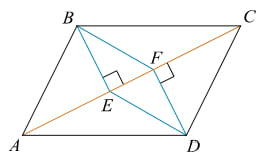
\includegraphics[align=t, width=\linewidth]{\picpath/G92M8L5}
		\end{minipage}
		\item В параллелограмме проведены биссектрисы противоположных углов. Докажите, что отрезки биссектрис, заключенные внутри параллелограмма, равны.
		\item Три стороны параллелограмма равны. Докажите, что отрезок с концами в серединах противоположных сторон параллелограмма равен четверти его периметра.
	\end{listofex}
\end{class}
%END_FOLD

%BEGIN_FOLD % ====>>_ Домашняя работа 3 _<<====
\begin{homework}[number=3]
	\begin{listofex}
		\item Домашняя работа 3
	\end{listofex}
\end{homework}
%END_FOLD

%BEGIN_FOLD % ====>>_____ Занятие 7 _____<<====
\begin{class}[number=7]
	\title{Подготовка к проверочной}
	\begin{listofex}
		\item Занятие 7
	\end{listofex}
\end{class}
%END_FOLD

=%BEGIN_FOLD % ====>>_ Проверочная работа _<<====
\begin{exam}
	\begin{listofex}
		\item Проверочная
	\end{listofex}
\end{exam}
%END_FOLD

%BEGIN_FOLD % ====>>_ Консультация _<<====
\begin{consultation}
	\begin{listofex}
		\item Сократите дроби:
		\begin{tasks}(2)
			\task \( \dfrac{2^{n+2}\cdot21^{n+3}}{6^{n+1}\cdot7^{n+2}} \)
			\task \( \dfrac{18^{n+3}}{3^{2n+5}\cdot2^{n-2}} \)
		\end{tasks}
		\item Расстояние между городами \( A \) и \( B \) равно \( 490 \) км. Из города \( A \) в город \( B \) со скоростью \( 55 \) км/ч выехал первый автомобиль, а через час после этого навстречу ему из города \( B \) выехал со скоростью \( 90 \) км/ч второй автомобиль. На каком расстоянии от города \( A \) автомобили встретятся?
		\item При смешивании первого раствора соли, концентрация которого \( 40\% \), и второго раствора этой же соли, концентрация которого \( 48\% \), получился раствор с концентрацией \( 42\% \). В каком отношении были взяты первый и второй растворы?
		\item Костя и Руслан выполняют одинаковый тест. Костя отвечает за час на \( 19 \) вопросов теста, а Руслан --- на \( 20 \). Они одновременно начали отвечать на вопросы теста, и Костя закончил свой тест позже Руслана на 9 минут. Сколько вопросов содержит тест?
		\item Постройте график функции
		\[y=	 \left\{
		\begin{array}{l}
			x-3, \quad x<3,\\
			-1,5x+4,5, \quad 3\le x\le4,\\
			1,5x-7,5, \quad x>4
		\end{array}
		\right. \]
		и определите, при каких значениях \( m \) прямая \( y=m \) имеет с графиком ровно две общие точки.
		\item  Постройте график функции
		\[y=	 \left\{
		\begin{array}{l}
			-x^2-4x-4, \quad x<-1,\\
			1-|x-1|, \quad x\ge-1
		\end{array}
		\right. \]
		и определите, при каких значениях \( a \) прямая \( y=a \) имеет с графиком ровно две общие точки.
	\end{listofex}
\end{consultation}
%END_FOLD

%BEGIN_FOLD % ====>>_ Консультация _<<====
\begin{consultation}
	\begin{listofex}
		\item \begin{minipage}[t]{\bodywidth}
			На стороне \( AC \) треугольника \( ABC \) выбраны точки \( D \) и \( E \) так, что углы \( ADB \) и \( BEC \) равны (см. рис.). Оказалось, что отрезки \( AE \) и \( CD \) тоже равны. Докажите, что треугольник \( ABC \) --- равнобедренный.
		\end{minipage}
		\gapwidth
		\begin{minipage}[t]{\picwidth}
			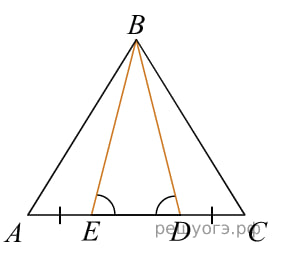
\includegraphics[align=t, width=\linewidth]{\picpath/G91M8C1}
		\end{minipage}
		\item В равностороннем треугольнике \( ABC \) точки \( M \), \( N \), \( K \) --- середины сторон \( AB \), \( BC \), \( CA \) соответственно. Докажите, что треугольник \( MNK \) --- равносторонний.
		\item Докажите, что у равных треугольников \( ABC \) и \( A_1B_1C_1 \) биссектрисы, проведённые из вершины  \( A \) и \( A_1 \), равны.
		\item В треугольнике \( ABC \) угол \( B \) равен \( 36\degree \), \( AB=BC \), \( AD \) --- биссектриса. Докажите, что треугольник \( ABD \) --- равнобедренный.
		\item Докажите, что медиана треугольника делит его на два треугольника, площади которых равны между собой.
		\item Сторона \( BC \) параллелограмма \( ABCD \) вдвое больше стороны \( CD \). Точка \( L \) --- середина стороны \( BC \). Докажите, что \( DL \) --- биссектриса угла \( CDA \).
		\item Докажите, что отрезок, соединяющий середины оснований трапеции, делит её на две равные по площади части.
	\end{listofex}
\end{consultation}
%END_FOLD

%BEGIN_FOLD % ====>>_ Консультация _<<====
\begin{consultation}
	\begin{listofex}
		\item Основания \( BD \) и \( AD \) трапеции \( ABCD \) равны соответственно \( 5 \) и \( 45 \), \( BD=15 \). Докажите, что треугольники \( CBD \) и \( BDA \) подобны.
		\item Точка \( K \) --- середина боковой стороны \( CD \) трапеции \( ABCD \). Докажите, что площадь треугольника \( ABK \) равна сумме площадей треугольников \( BCK \) и \( AKD \).
		\item В треугольнике \( ABC \) с тупым углом \( ABC \) проведены высоты \( AA_1 \) и \( CC_1 \). Докажите, что треугольники \( A_1BC_1 \) и \( ABC \) подобны.\\
		\item Сторона \( AB \) параллелограмма \( ABCD \) вдвое больше стороны \( AD \). Точка \( K \) --- середина стороны \( AB \). Докажите, что \( DK \) --- биссектриса угла \( ADC \).
	\end{listofex}
\end{consultation}
%END_FOLD